\begin{wrapfigure}{r}{0.55\linewidth}
	  \begin{center}
	    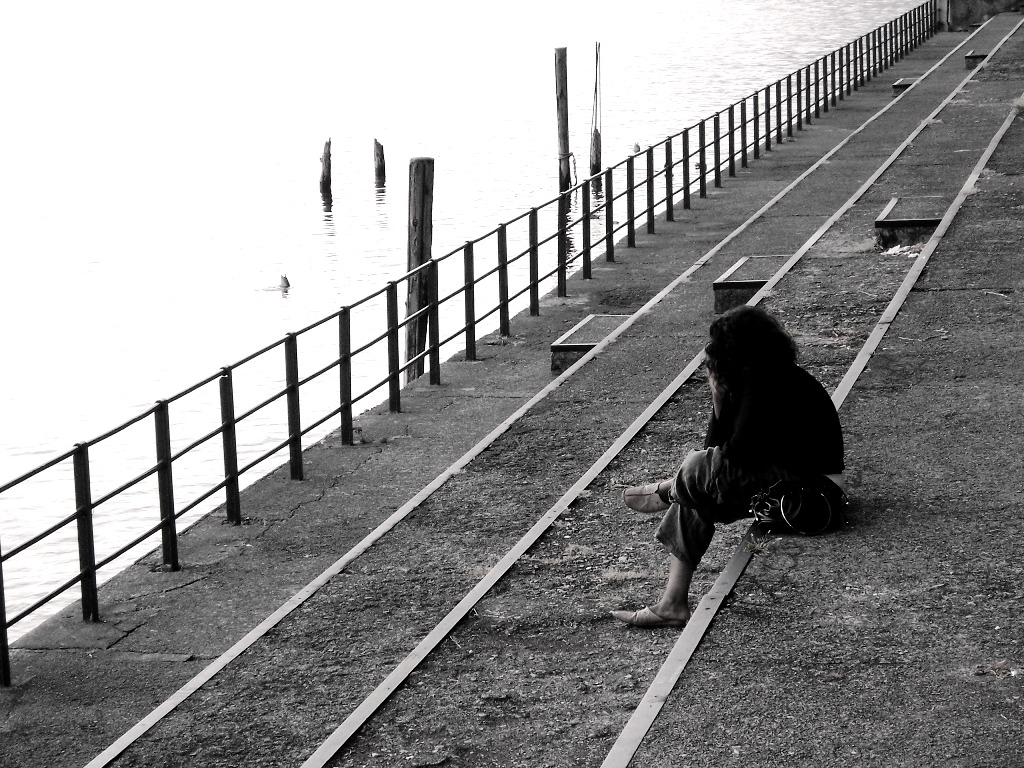
\includegraphics[width=0.9\linewidth]{images/waiting}
			\captionsetup{labelformat=empty,justification=centering}
	    \caption{Waiting.}
	    \label{medio:waiting}
  \end{center}
\end{wrapfigure}

At this point, we have learned a few things about both electronics and programming. Learning that we can write code that expresses ideas regarding parallelism with \PAR is, we think, a fundamental and world-changing concept for many programmers. If it felt ``natural,'' that's a good thing. 

\begin{comment}
	\begin{figure}[h!]
	  \begin{center}
	  \end{center}
	\end{figure}
\end{comment}

In terms of electronics, we learned how to connect an LED to our Arduino. In terms of programming, we learned some of the basics of the syntax of \occam. Next, we're going to learn a bit about {\em waiting} and {\em signaling}. Like everything else about \plumbing, we'll do this in \PARallel---one process will be responsible for signaling that something has changed (a button is pressed, for example), while another waits to see what has happened.




